\documentclass[aspectratio=169]{beamer}              % only frames

% for themes, etc.
\mode<presentation>
\usetheme{Madrid} 
\usecolortheme{crane}

%\usepackage{times}  % fonts are up to you
% The usual suspects
\usepackage{multirow, booktabs, dcolumn, color, graphicx} % Tables\usepackage{graphicx}
\usepackage{amsmath,amssymb,amsthm}
% Strikethrough text
\usepackage{soul}
% Adjust box to fit tabulars
\usepackage{adjustbox}
% Embed video
\usepackage{media9}
% For notes
\usepackage{pgfpages}
\setbeameroption{hide notes} % Only slides
%\setbeameroption{show only notes} % Only notes
%\setbeameroption{show notes on second screen=right} % Both
% Use colors by name
\usepackage{xcolor}
% EMBEDDING VIDEO IS POSSIBLE WITH PDFPC USE PDF PC to present
\usepackage{multimedia}



% The table highlighting for hypothesis discussion.
\usepackage[beamer,customcolors]{hf-tikz}
\usetikzlibrary{calc}

% To use background images
\newenvironment{colorframe}[2][]{%
\setbeamercolor{background canvas}{bg=#1}
\begin{frame}\color{white}}
{\end{frame}}


% To set the hypothesis highlighting boxes red.
\tikzset{hl/.style={
    set fill color=red!80!black!40,
    set border color=red!80!black,
  },
}

% Set Graphics folder
\graphicspath{{./figures/}}


% these will be used later in the title page
\title{Cryptography}
\subtitle{Asymmetric Key Cryptography}
\author{Irfan Kanat}
\institute[CBS]{{Department of Digitization}\\ Copenhagen Business School}
%\date{\today}



\begin{document}

% this prints title, author etc. info from above
\begin{frame}

	\titlepage


	\vfill
	{\tiny \centering This work is licensed under a \href{http://creativecommons.org/licenses/by/4.0/}{Creative Commons Attribution 4.0 International License}.}

\end{frame}

\note{In this presentation we focus on asymmetric key cryptography and how it is used to ensure Confidentiality, Integrity, and Authentication.}


\begin{frame}
	\frametitle{Recap: Symmetric Key Cryptography}

	\centering

	{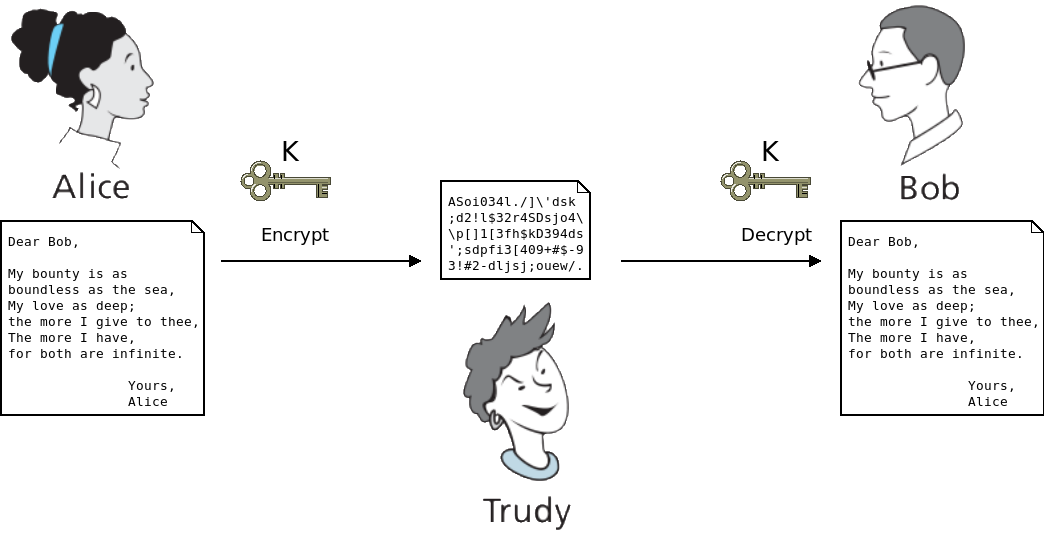
\includegraphics[width = \textwidth, height = .85\textheight, keepaspectratio]{figures/symmetricEncExample.png} }
	
\end{frame}

\note{If Alice and Bob have met before and shared a key,

Then they can encrypt and decrypt their messages without Trudy getting any wiser.

A single key both locks and unlocks the box and reveals the tender words of our office lovers.
}


\begin{frame}
	\frametitle{The Problem with Symmetric Key Cryptography}

	For two thousand years cryptography required a shared key. \vspace{1em}

	This is ok if you can meet and exchange keys. \vspace{1em}

	Did you exchange keys with your bank?

\end{frame}

\note{
	Symmetric Key cryptography is perfectly fine if you can share keys with the other party.

	Yet there are so many use cases where we need to communicate with parties that we won't meet.

	An example was submarines leaving for months long voyages during world war II. For other troops that were part of the network, new keys could be sent via courier. The submarines had to store keys in advance. This made them a target.

	A less exciting but still more relevant case is websites. You often see the green lock icon in the address bar. Indicating you are communicating with the right party and your communications are secured. But you have not exchanged keys with every web site in the world... 

	How come you can tell you are talking to your bank and not some scammers? How come you can be sure your information is encrypted?
}

\begin{frame}[t]
	\frametitle{Big Idea: Securing Data in Transit}

	Alice and Bob want to communicate securely \vspace{1em}

	\begin{itemize}
		\item Confidentiality
		\item Integrity
		\item Authentication
	\end{itemize}
    
\end{frame}

\note{
	It is fine to encrypt and decrypt the data with a single key if that data is sitting on your devices, when you want to exchange data through an unreliable medium (such as internet) you need to consider a few things.

	Principles of secure communications.

	AGAIN CIA but a different A this time.

	Confidentiality: That Trudy can not read your love letters.

	Integrity: That Trudy can not alter your love letters.

	Authentication: That Trudy can not pretend to be Alice.
}



\begin{frame}[t]
	\frametitle{Asymmetric Key Cryptography}
    
    \begin{columns}
		\begin{column}{0.5\textwidth}

		We shared keys for 2000 years \vspace{1em}

		\only<2->{Then we found a better way! \vspace{1em}}

		\only<3->{RADICALLY DIFFERENT! \vspace{1em}

		MARVELOUSLY ELEGANT!}
	
		\end{column}

		\begin{column}{0.5\textwidth}

			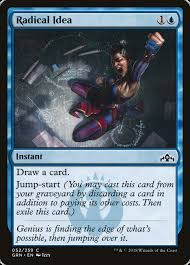
\includegraphics[width = \textwidth, height = .85\textheight, keepaspectratio]{figures/radicalIdea.jpeg}

		\end{column}

	\end{columns}

\end{frame}

\note{Sharing keys is so 1970. 

In 76, we found a better idea.
}

\begin{frame}
	\frametitle{Asymmetric Key Cryptography}

	\centering

	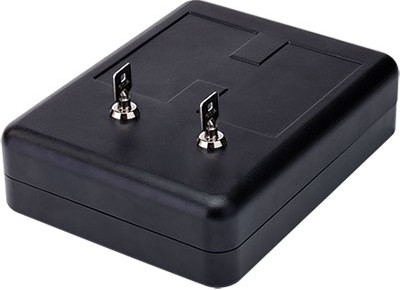
\includegraphics[width = \textwidth, height = .85\textheight, keepaspectratio]{figures/LockBox2.png}

\end{frame}

\note{
	WHAT IF WE ADD ANOTHER KEY?

	Two separate keys to secure data.

	Whatever you lock with one key, can only be unlocked with the other.

	It is not immediately apparent how this is an improvement but bear with me and I will show you what it means in terms of secure communications.
}



\begin{frame}
	\frametitle{Keys Galore!}

	Everyone gets two keys! \vspace{1em}

	\begin{itemize}
		\item Public Key
		\item Private Key
	\end{itemize}
    
\end{frame}

\note{EVERYONE GETS TWO KEYS!

A PUBLIC KEY THAT YOU SHOUT OUT FROM ROOF TOPS. YOU WANT THE WORLD TO KNOW. (K+)

and a private key, you hold close to your heart and not even share with your dearest. (K-)

The wallet addresses of crypto currencies for example are public keys. You can't spend the money in the wallet without the private key.

}


\begin{frame}
\frametitle{PKE and Secure Communications}

Let's remember:\vspace{2em}

	\hspace{1em} Confidentiality \vspace{1em}

	\hspace{1em} Authentication \vspace{1em}

	\hspace{1em} Integrity\vspace{2em}

How can we achieve these with PKE?

\end{frame}


\begin{frame}[plain]
\frametitle{Confidentiality}


\only<1>{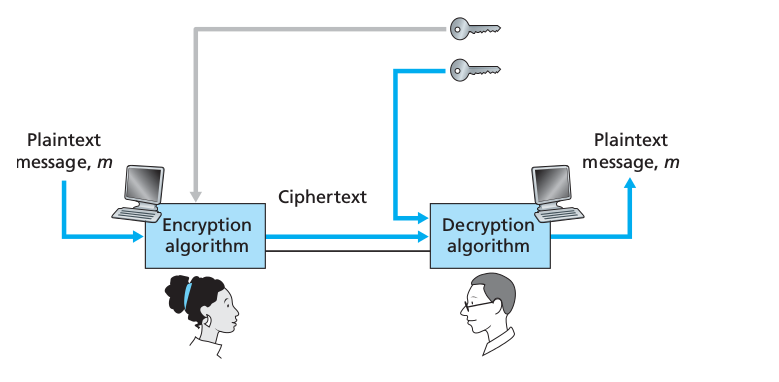
\includegraphics[width = \textwidth, height = .85\textheight, keepaspectratio]{figures/Confidentiality.png}}

\only<2>{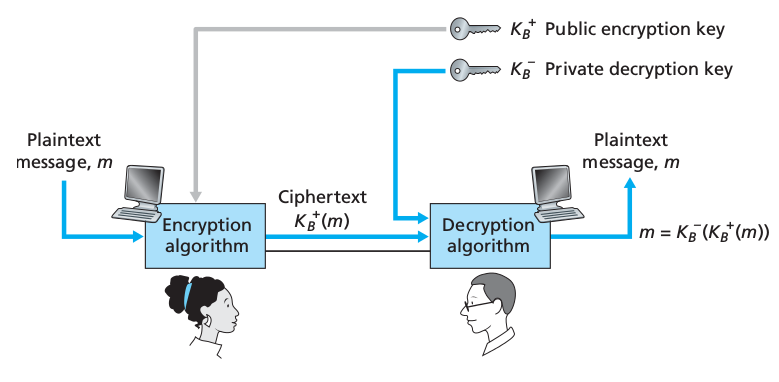
\includegraphics[width = \textwidth, height = .85\textheight, keepaspectratio]{figures/Confidentiality2.png}}

\end{frame}
\note{

How can you ensure only the intended receiver can read your messages? \vspace{1em}

You have three keys in your hand. Your private/public key pair and your destination's public key pair. So you have three options.

You need to choose a key that threat actors (Trudy) along the way don't posses. So that your message gets accross unread.
}


\begin{frame}[plain]
\frametitle{Authentication}

\only<1>{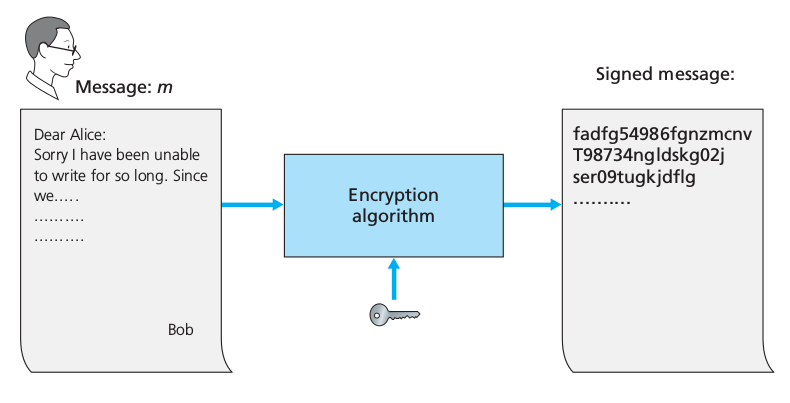
\includegraphics[width = \textwidth, height = .85\textheight, keepaspectratio]{figures/authentication.png}}

\only<2>{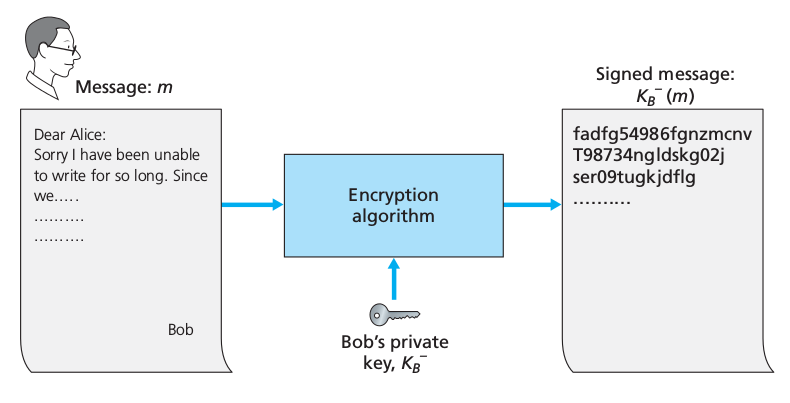
\includegraphics[width = \textwidth, height = .85\textheight, keepaspectratio]{figures/authentication2.png}}
\end{frame}

\note{

How can you make sure the receiving party knows for sure that you are indeed the sender?

Here you don't care if they can read the message or not. All you care about is if they can make sure it is you.

Again you have three keys in your hand, your own pair, and your destination's public key.

You need to pick a key that nobody else possesses, but everyone else can undo and prove that it was indeed locked by you.
}



\begin{frame}
\frametitle{Integrity and Digital Signatures}

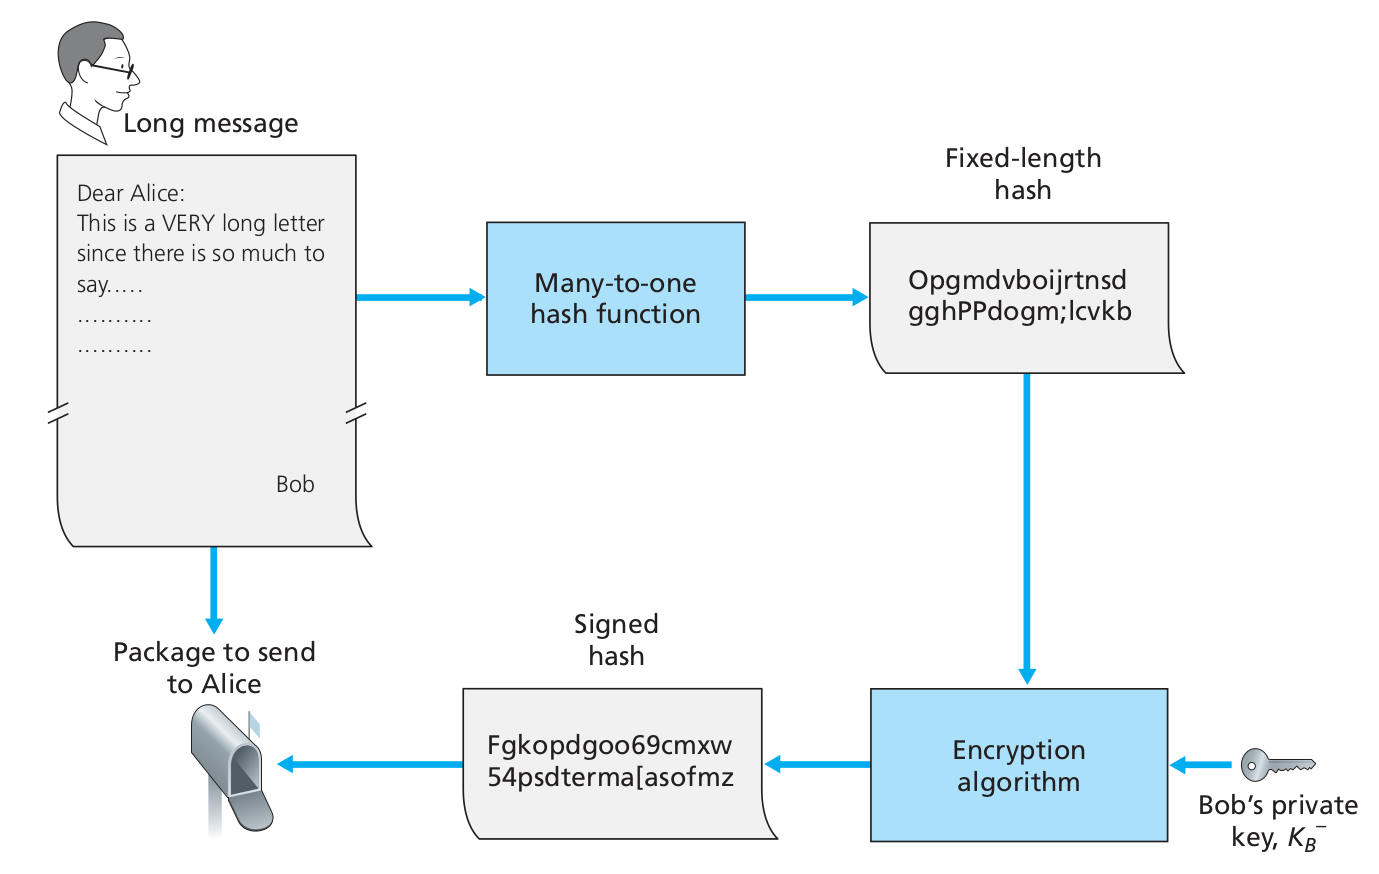
\includegraphics[width = \textwidth, height = .85\textheight, keepaspectratio]{figures/digitalSignature.png}

\end{frame}

\note{Before we get into it, here is something you need to know. A hash function is essentially a function that takes a long message and creates a short summary version of it. When you feed the same message, it always produces the same output.

Integrity: We want to make sure the message was unaltered.

Sometimes you may need to broadcast a message. You don't care about confidentiality at all, infact you want everyone to be able to read the message. Like when you publish software on the internet. BUT! it is important to make sure the message is not changed and is indeed the same message you wrote. Like nobody inserted a virus into the software you published.


So you send the message, and encrypt a summary of the message with your private key (authenticating it is indeed you). That encrypted summary is called a digital signature.

Using your public key, anyone can make sure the hash they obtain from the message matches the one in your signature.

This is how we can make sure a message's contents are unaltered.}


\begin{frame}
	\frametitle{Certificates and Certificate Authorities}
    
    \only<1>{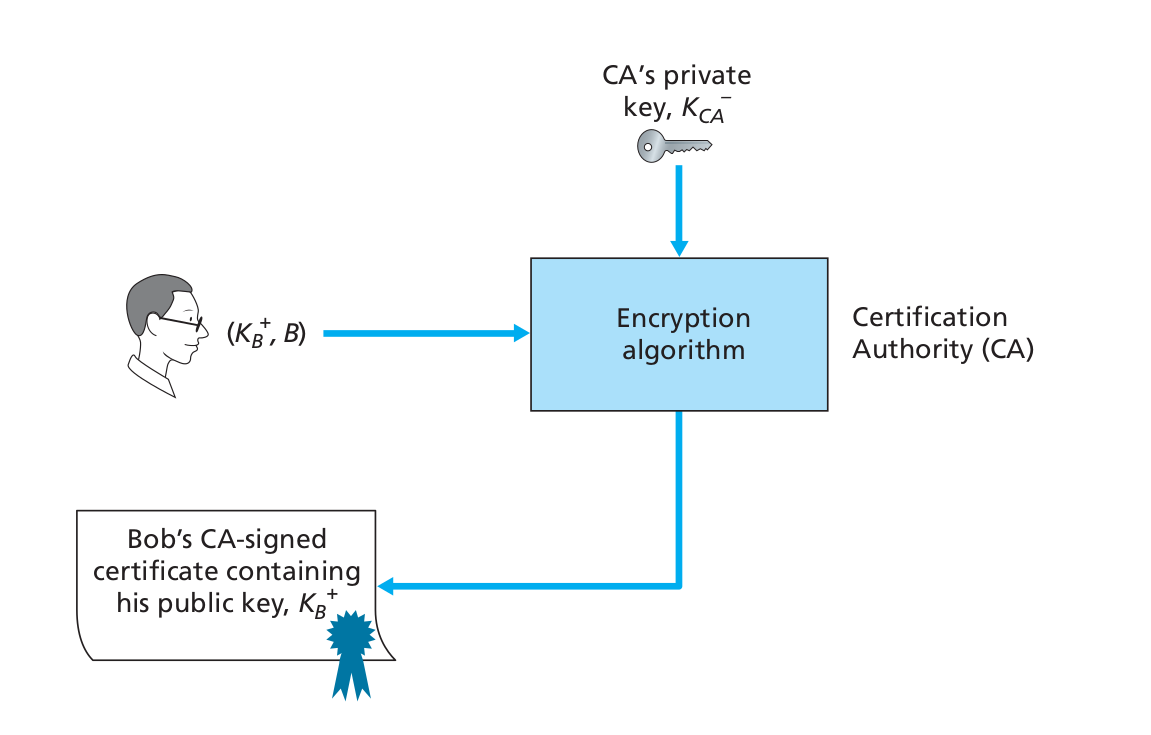
\includegraphics[width = \textwidth, height = .85\textheight, keepaspectratio]{figures/CertificateAuthority.png}}
    \only<2>{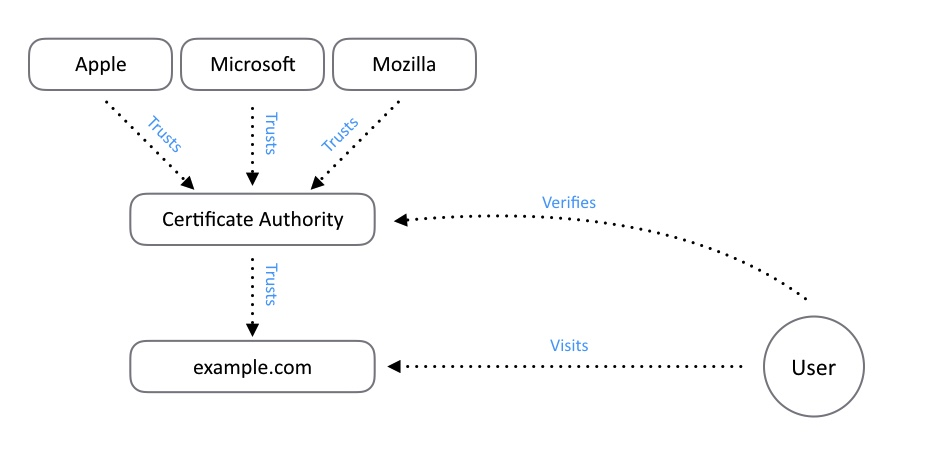
\includegraphics[width = \textwidth, height = .85\textheight, keepaspectratio]{figures/TLSIntercept0.jpeg}}

\end{frame}

\note{For it all to work, we need a reliable way to distribute public keys.

As anyone can create key pairs, we need to associate public keys with identities/entities.

That is where trusted third parties called Certificate Authorities come in.

CA's public keys are widely known. These are often bundled with operating systems and other relevant software.

When you register with a CA, they sign your public key. So anyone can verify that the public key was registered with a CA. 

The signed public key (and a few details on identity) is called a certificate.

When you browse to your bank's website they send you one such certificate. So you can use CA's public key to decrypt the certificate and obtain the bank's public key.}


\begin{colorframe}[black]

	\centering
	\Large
	Certificate Authorities, what could go wrong?

\end{colorframe}

{
\usebackgroundtemplate{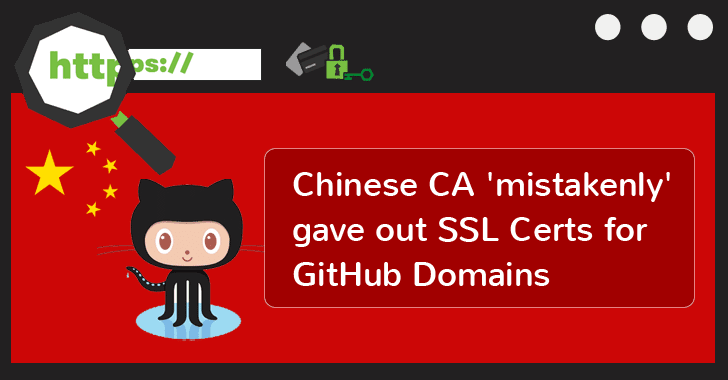
\includegraphics[width=\paperwidth,height=\paperheight]{figures/github-ssl-certificate.png}}%
	\begin{frame}
	\frametitle{}

	\end{frame}
}

\note{
	
	If there is a CA out there with wide spread acceptance.

	They may abuse their position to facilitate man in the middle attacks.

	Or if the CA does not practice due diligence, they may ``accidentally'' provide certificates for a domain already registered.

	Multiple governments that have control of a Certificate Authority have issued certificates that can allow them to eaves drop on encrypted communications in the past (Kazakhstan, India, China...).

}


\begin{frame}
	\frametitle{Asymmetric Key Cryptography and Data in Transit}

	Ideal for communication \vspace{1em}

	Overhead is a problem \vspace{1em}

	In combination with Symmetric key encryption. \vspace{1em}

\end{frame}

\note{As we have seen, the nature of PKE makes it useful for securing communications.

Yet the computational overhead of PKE makes it slow for real time applications.

Hence in reality, PKE is only used to authorize and exchange shared keys. 

Once two sides share keys through, PKE, they switch to symmetric key cryptography for the rest of the session.}


\begin{frame}
	\frametitle{Recap}
    
    \begin{itemize}
    	\item The Need for Multiple Keys
    	\item Asymmetric Key Cryptography
    	\item Confidentiality, Integrity, and Authentication (the other A)
    \end{itemize}

\end{frame}

\note{Internet is a jungle. It can be beautiful but you need to watch out for yourself. Things you do online have consequences IRL.}

\end{document}
